\subsection{Ranking Within the Degree Equalises Access with a Small Observed Grade Difference}
\label{sec:res-rules}

Ranking students within their degrees makes their chances of selection much more similar. Among the 3,469 students with grades in both semesters, the last panel of Figure~\ref{fig:rules} shows the standard deviation of selection rates falling from 0.090 under raw GPA (95\% interval 0.082--0.107) to 0.006 under percentiles (0.005--0.013). Regression adjustment and within-degree $z$-scores fall between them, at 0.040 and 0.019. The earlier exercise with all 3,703 students illustrates what this means: selection rates range from 5\% to 36\% under raw grades, compared with 19\% to 21\% under percentiles. In that larger sample, the within-degree rules change 138--156 of the 741 places.

\begin{figure*}[t]
  \centering
  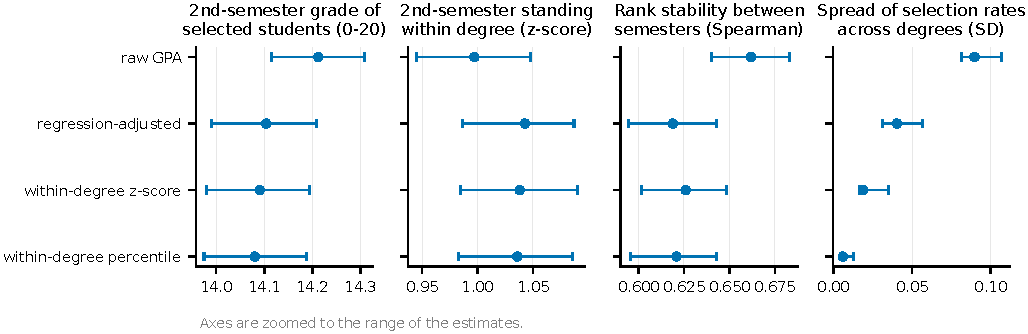
\includegraphics[width=\textwidth]{fig6_ranking_rules}
  \caption{Four rules selecting the top 20\% of 3,469 Portuguese students using first-semester grades, evaluated against second-semester outcomes, entry profile and selection balance. Bars show 95\% intervals from 1,000 student bootstrap resamples. Grade points use the 0--20 scale; standardised measures use standard-deviation units, and selection rates are proportions. Axes are zoomed: the raw-grade difference in the first panel is 0.13 points. Original figure; records from Realinho et al.}
  \label{fig:rules}
\end{figure*}

The difference in later grades is much smaller. Students selected by raw GPA average 14.21 in the second semester (14.11--14.31), compared with 14.08 under percentiles (13.97--14.19). That is a gap of 0.13 points on a 0--20 scale. The intervals overlap, although this alone does not prove that the rules perform equally or test the difference between them. If we look instead at students' standing within their degrees, the percentile rule comes out slightly ahead: the average standardised second-semester grade is 1.04, compared with 1.00 under raw GPA. Which result matters more depends on whether we want to reward reported grades or performance relative to classmates. Neither measure independently tells us how much students have learnt.

Raw GPA produces a more stable ranking between semesters, with a correlation of 0.66 compared with 0.62 for percentiles. However, grade differences between degrees can repeat too, contributing to that stability. A stable ranking is therefore not necessarily a more accurate measure of individual achievement. The selected students' mean standardised admission grades are 0.55 under raw GPA and 0.48 under percentiles, with overlapping intervals of 0.46--0.63 and 0.39--0.56. In this institution, percentiles give students much more similar chances across degrees, while the selected groups have broadly similar entry profiles and later grades.
